\section{Timeline}

The following section describes the project development, progress and decision as we did through the time the the project was developed. After series of informal talk the project officially started in December 2011 and was submitted in September 2012.

\subsection{Initial project meetings and early implementation decisions}

The regular project meeting where we discussed mostly the organizational aspects and the top-level design of the application started in December 2011. We easily agreed that we were aiming to create an application quite similar to the Google Documents. We have decided very early to use the multi tier architecture consisting of

\begin{itemize}
\item core translation memory,
\item user space,
\item graphical user interface,
\end{itemize}

which became very soon separate Maven modules (as soon started using Maven for building the project). Despite we added further modules later, we consistently kept the initial project splitting into \emph{Core}, \emph{User Space} and \emph{GUI}. At the beginning we also assigned team members to the different part of project which remained surprisingly stable as well. 

Before receiving the data from OpenSubtitles.org we were thinking about the source of data to fill the translation memory for the first time. There were several options -- either using the subtitle part of the Czech-English parallel corpus CzEng developed at ÚFAL, using sentences from a general purpose parallel corpus or getting the data from a subtitle server.

From the very beginning we intended base the project on Java. Mainly because there exist quite a lot of web technologies based on Java and everybody of us were at least a little bit familiar with it. We also decided to combine the code in Java and Scala programming languages and Apache Maven as a build manager. At that time there was only one team member who knew the Scala language. Despite we repetitively expressed believes that everybody of would learn it, at the end there was one another person familiar with the Scala language which appeared to be a bottleneck of work on the translation memory core.

Much complicated was to agree on the technology of the client. There were many different opinions from writing the client in {\it PHP} with {\it Nette Framework} which some of us know quite well, using the {\it JSP} to have all the code consistently in Java or even quite extreme idea to make the whole application as {\it Java Applet} (this idea had appeared because of the intention to integrate the video player in the application and at that time we didn't of any other option of doing it except making a Java applet for it). Finally we decided to use {\it Google Web Toolkit} which nobody of us had had any prior knowledge before, but it promised making the communication between server and client very easy. Similarly to the Scala language we ended up with just two people able to work effectively with the Google Web Toolkit. Fortunately, it did not became a bottleneck of the development process. 

After overcoming the problems connected with learning a new technology we became quite satisfied with the decisions because the usage of Google Web Toolkit and other modules, as well as the possibility to combine all parts of the project with Apache Maven were helpful despite making the project run in Maven was very painful for us and we spent unnecessarily a lot of time by solving this issues.
	
The decision to use both Java and Scala appeared to be a bring quite a lot of complications. On the one hand, Scala allowed to write concise and efficient code, on the other hand most project members were not able to learn Scala sufficiently and hence used only Java. Although the interoperability between Scala and Java works well in most cases because both are based on the JVM, some problems remain. One of the problems of interoperability was, for example, that the implementation of the data type \emph{List} that was created in Scala was not compatible with Google Web Toolkit, which expected a standard Java \emph{List} implementation.

\subsection{Early development process}

Luckily for us we received very soon a database from the {\it opensubtitles.org} containing all the Czech and English subtitle file that were at the server at that time. Soon after that we started an alignment algorithm to retrieve the parallel data from the subtitle files (the process is described in section~\ref{sec:aligning_subtitles}) and enable us to start experiments that helped us to decide which database system could be used.

Choosing appropriate database system was also intensively discussed issue. The database underlying the Translation Memory plays a crucial role for the whole system performance. Also using built-in features could save us a lot of additional work.  We evaluated different DBMS and decided to use Postgres (see section~\ref{sec:dbms} for details). Not having any experience with the object-relation mapping libraries in Java we started to us {\it Hibernate} based on the Internet forums and advice of our colleagues.

Originally, all the algorithms precessing the data we retrieved were implemented in Perl the and the code importing the data were in the \emph{Core} module implemented in Scala. Later, to be the code more consistent, we decided to move the data preparation and data import to a separate \emph{dataimport} module and re-implement the Perl scripts in Scala.

\begin{figure}[h]
\begin{center}
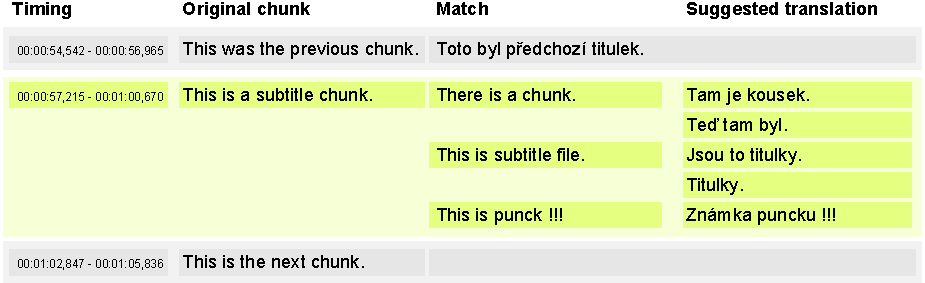
\includegraphics{./figures/original_strucutre.pdf}
\end{center}

\caption{Scheme of the originally intended structure of work with the translation memory. It reflects the original User Space structure and also schematically the original client design.}\label{fig:original_scheme}

\end{figure}

We started to solve very soon the video playback in the browser which we expected to be a really challenging issue. ... we thought about flash, creating application wrapper where an web would be included ...

\subsection{Introducing the shared classes}

After having implemented very basic version of both three parts of the project we decided it was time to start to solve the interoperability of individual parts in order run a first snapshot of the application. This was happening approximately in March 2012.

At this stage we found out that we are not fully taking advantage of using the Java technologies for all parts of project and decided to totally redesign the User Space and Client parts.

Originally we wanted to keep the traditional translation memory structure where each sentence can have several matches and these matches can have several translations in the memory as is depicted in the figure \ref{fig:original_scheme}. Anyway, this scheme did not reflect much the way we worked with the data in the that time -- suitable matches were provided from the table of translation pairs based on indexes built over the table. Moreover, the were very few matches having more different translations in the data and the design of the GUI of the application was a little bit confusing because it used to place the text of matches to prominent place despite the user is not as concerned about the matches as he is about the actual translation suggestions. This lead to a scheme which is depicted in figure \ref{fig:new_scheme}.

\begin{figure}
\begin{center}
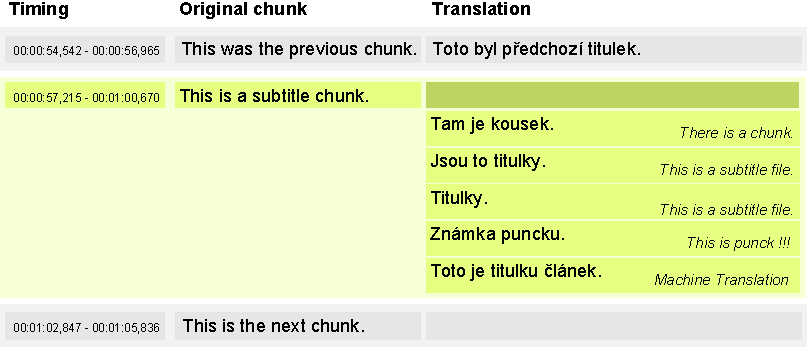
\includegraphics{./figures/current_strucutre.pdf}
\end{center}
\caption{Current scheme of the work with translation memory.}\label{fig:new_scheme}
\end{figure}

We agreed on the shared classes that all parts of the project should use.  We more or less adopted the design of the class from the core and started to use in the whole project. This step required to re-implement the classes from Scala to Java and to drop a lot of code that was already done in the User Space and the client. The design of the classes was almost the same as is described in \ref{sec:shared_structure}.

We started the work on the project with new design soon, anyway it started the period of the biggest struggle with technologies. It took almost two months to have a first running version of the application.

The very first version of the application was a page where it was possible to upload a subtitle file do the translation without any possibility load an already saved subtitle document or download a result of the translation. without any sessions, user, it was just a page, where you edit the subtitles. At that time we used machine translation from the MyMemory service which is in fact Google Translate, anyway there is a limited acces per IP address, so it became obvious the we would have to change the source of machine translation. We used API of IMDB.com, to receive information about movies but the movie meta data was not used in the evaluation the matches at that time.

From the later view it appeared to be an important decision to agree on the shared classes which made the cooperation between the modules easier and less verbose. 

\subsection{???}

Sessions, logging, troubles with OpenID, trying JOpenID, openid4java 

Use our own Moses trained on the subtitle data we have from opensubtitles

\subsection{Final Development}

Optimizations required: better to throw away translation pairs and generated everytime user logs in

Found many technical issues: e.g. necessary to be able to stop loading generating the suggestions on the server at the moment

We left to the end a lot issues which we considered to be only minor technical , which appeared to be a lot of intensive work.

We estimated the 12$^\mathrm{th}$ August, 12 p.m. to be a day that we called the Feature Freeze which meant that after this date no new features were added to the project. At that time we started an intensive review of already existing code, debugging and working on the documentation. 

\section{Evaluating the Development Process}

One of the crucial decision for the project was the choice of technologies. Most of the technologies we used -- Maven, Scala, Hibernate, GWT -- were new to all of us and we also had not much experience with the other. Combining these technologies together was quite painful and would probably even for an experienced Java developer. Generally, we can say that the fact that we were not too much familiar with the technologies, we spent most of the time solving technical issues. There is quite a lot of research challenges, mostly in the fuzzy matching part, which had to remain untouched due to that.

On the other hand the choice of technologies appeared to be lucky that it probably saved a lot of work for us by the possibility to share implementation of class. Using the Scala language for the core also made the parallelization much easier.

Despite we spent quite a lot of time by the discussions how the structure of the project we didn't avoid a radical change of the design of the application 4 months after the project started. Nearly the whole User Space code had to be dropped and it was also necessary to totally remake the client components existing so far.

A bottleneck of the development process was also that not all of us were familiar with all of the technologies. It happened many times that somebody could not continue developing a particular part of the project and had to wait for an other team member to fix the issue even though it may have been just changing a single attribute in the Hibernate mapping.

Problems with communication, different communication platforms among time, members of the team sometimes must have waited for othres...



